%\usepackage{subfigure}
%\usepackage[usenames,dvipsnames]{color}
\newcommand{\blue}{\color{blue}}
\newcommand{\htr}[1]{{\color{red} #1}}
\newcommand{\htb}[1]{{\color{blue} #1}}
\newcommand{\htg}[1]{{\color{green} #1}}
\newcommand{\htrd}[1]{\htr{\st{#1}}}
\newcommand{\htbd}[1]{\htb{\st{#1}}}
\newcommand{\htgd}[1]{\htg{\st{#1}}}
%\newcommand{\cb}{\color{blue}}
%\newcommand{\cred}{\color{red}}
%\newcommand{\cblack}{\color{black}}
%\newcommand{\nn}{\nonumber}
%\usepackage{minipage}
%\usepackage{axodraw}
%\captionsetup[subfloat]{captionskip=-0.7cm,labelfont=bf,font=normalsize} 
%\renewcommand{\topfraction}{0.99}       % max fraction of floats at top
%\renewcommand{\bottomfraction}{0.99}    % max fraction of floats at bottom
%\renewcommand{\textfraction}{0.01}      % allow minimal text w. figs
%\newcommand{\TeV}{{\ensuremath\rm TeV}}
%\newcommand{\GeV}{{\ensuremath\rm GeV}}
%\newcommand{\MeV}{{\ensuremath\rm MeV}}
%\newcommand{\fb}{{\ensuremath\rm fb}}
%\newcommand{\pb}{{\ensuremath\rm pb}}
\newcommand{\eqn}{equation}
\newcommand{\al}{\alpha}
%\newcommand{\be}{\beta}
\newcommand{\lb}{\left(}
\newcommand{\rb}{\right)}
\newcommand{\mO}{\mathcal{O}}
%\newcommand{\lam}{\lambda}
\def\met{{\slash\!\!\!\!\!\:E}_T}
\def\mpt{{\slash\!\!\!\!\!\:P}_T}
\def\metv{{\slash\!\!\!\!\!\:\vec{E}}_T}
\def\mptv{{\slash\!\!\!\!\!\:\vec{P}}_T}
\def\D0{\slash\!\!\!\!\!\!\!\!\!\:D0}
\newcommand{\HS}{\texttt{HiggsSignals}}
\newcommand{\HB}{\texttt{HiggsBounds}}
\newcommand{\HSv}[1]{\texttt{HiggsSignals-#1}}
\newcommand{\HBv}[1]{\texttt{HiggsBounds-#1}}

\newcommand{\cp}{\mathcal{CP}}
\newcommand{\MHexp}{125\,\GeV}
\newcommand{\ca}{\cos \alpha}
\newcommand{\csqa}{\cos^2 \alpha}
\newcommand{\sa}{\sin \alpha}
\newcommand{\ssqa}{\sin^2 \alpha}
\newcommand{\ssmlhc}{\sigma_\text{SM}^\text{LHC8}}
\newcommand{\tb}{\tan\beta}
\newcommand{\MHav}{\overline{M}_{12}}

%cite summaries
\newcommand{\oblique}{Altarelli:1990zd,Peskin:1990zt,Peskin:1991sw,Maksymyk:1993zm}
\newcommand{\m}{m_{H^{\pm}}}
\newcommand{\g}{\,\mbox{GeV}}
\newcommand{\la}{\lambda_1}
%\newcommand{\lb}{\lambda_2}
\newcommand{\lc}{\lambda_3}
\newcommand{\ld}{\lambda_4}
%\newcommand{\lp}{\lambda_5}
\newcommand{\lcz}{\lambda_{45}}
\newcommand{\lczp}{\lambda_{345}}
\newcommand{\rg}{R_{\gamma\gamma}}
\newcommand{\rgt}{\widetilde{R}_{\gamma\gamma}}
\newcommand{\fr}{\frac}
\newcommand{\relic}{\Omega_{DM}h^2}

\section{Inert Doublet Model}

The Inert Doublet model \cite{Deshpande:1977rw,Cao:2007rm,Barbieri:2006dq} is another intriguing model that extends the scalar sector of the Standard Model, providing dark matter candidates. It contains two scalar doublets $\Phi_S,\Phi_D$, redering five physical states $h,H,H^\pm,A$, where $h$ corresponds to the Standard Model Higgs particle and all other states originate from the second doublet. An additional $Z_2$ symmetry is imposed, with the discrete transformations defined as
% given by 
%\begin{equation}
$ \phi_D \to - \phi_D, \,\,
\phi_S\to \phi_S, \,\,
\text{SM} \to \text{SM}.$
%\end{equation}
This leads to the following potential. \begin{equation}\label{pot}\begin{array}{c}
V=-\fr{1}{2}\left[m_{11}^2(\phi_S^\dagger\phi_S)\!+\! m_{22}^2(\phi_D^\dagger\phi_D)\right]+
\fr{\lambda_1}{2}(\phi_S^\dagger\phi_S)^2\! 
+\!\fr{\lambda_2}{2}(\phi_D^\dagger\phi_D)^2\\[2mm]+\!\lambda_3(\phi_S^\dagger\phi_S)(\phi_D^\dagger\phi_D)\!
\!+\!\lambda_4(\phi_S^\dagger\phi_D)(\phi_D^\dagger\phi_S) +\fr{\lambda_5}{2}\left[(\phi_S^\dagger\phi_D)^2\!
+\!(\phi_D^\dagger\phi_S)^2\right],
\end{array}\end{equation}
with all  parameters real
(see e.g. \cite{Ginzburg:2010wa}).
After minimization, the model contains in total 7 free parameters which e.g. can be chosen as $(m_H,m_A,m_{H^{\pm}}, \lambda_2, \lambda_{345})$, where $\lambda_{345}\,\equiv\,\lambda_3+\lambda_4+\lambda_5$. The above $Z_2$ symmetry renders the lightest of the additional scalars stable, and the model therefore provides a good dark matter candidate. The following discussion focuses on $H$ as the dark matter candidate. The model is subject to a large number of theoretical and experimental constraints, cf. e.g. \cite{Dolle:2009ft,Swiezewska:2012eh,Arhrib:2013ela,Krawczyk:2013jta,Ilnicka:2015jba,Diaz:2015pyv,deFlorian:2016spz,Belyaev:2016lok,Ilnicka:2017gab,Eiteneuer:2017hoh} for recent discussions on the allowed parameter space. Most stringent constraints stem from direct detection experiments such as LUX \cite{Akerib:2016vxi} for large parts of the parameter space.

Due to the $Z_2$ symmetry, all scalars that originate from the second (dark) doublet can only be pair-produced. In addition, these dark scalars do not couple to fermions. The most prominent production channels are therefore Drell-Yan induced processes, i.e. the production of a single $W$ or $Z$ in the s-channel producing a pair of dark scalars. In principle $AA$ final states can also be mediated via an $h$ in the s-channel; however, the according couplings are strongly constrained from direct detection experiments, rendering the according contribution to the total cross section negligible. Therefore, the production cross sections for this model only depend on electroweak couplings as well as the masses of the produced dark scalars. Similarly, the dark scalars dominantly decay via $A\,\rightarrow\,Z\,H$ and $H^\pm\,\rightarrow\,W^\pm\,H$, with electroweak gauge bosons following SM decay patterns.

Total cross sections for scans as well as dedicated parameter points have been presented in \cite{Ilnicka:2015jba,deFlorian:2016spz,Belyaev:2016lok}. Typical production cross sections for $Z+\MET$ or $W^\pm\,+\,\MET$ at the 13 TeV LHC are of the order of 30 fb, where no cuts have been applied. Production cross sections for diboson final states and $\MET$ are suppressed by an additional factor 3-10\footnote{In principle, also monojet searches could render insight on this model. However, the according production cross sections are proportional to $\lambda_{345}^2$. The value of this parameter is highly constrained by direct detection experiments.}.

The UFO model file for the Inert Doublet Model has been presented in \cite{Goudelis:2013uca} and can readily be interfaced with Madgraph to produce event samples at all levels. Collider studies of this model at the LHC as well as a Linear Collider framework have e.g. been discussed in \cite{Gustafsson:2012aj,Arhrib:2013ela,Hashemi:2015swh,Poulose:2016lvz,Datta:2016nfz,Hashemi:2016wup}.

For the most dominant production channels, i.e. mono gauge-boson production with missing energy, the production mode differs from the model discussed above, cf. Figure \ref{fig:haprod} (the diagram for $H^\pm\,H$ production is analogous). Both the nature of the s-channel mediator as well as the decay topology differ. Therefore, although final state signatures are identical within the two models, it can be expected that different selection cuts need to be applied for signal enhancement. Possible search strategies can e.g. be adopted from improvements of experimental cuts for supersymmetric searches in multilepton final states (see \cite{Belanger:2015kga} for a recast of this model using 8 \TeV LHC data).
\begin{figure}
\centering
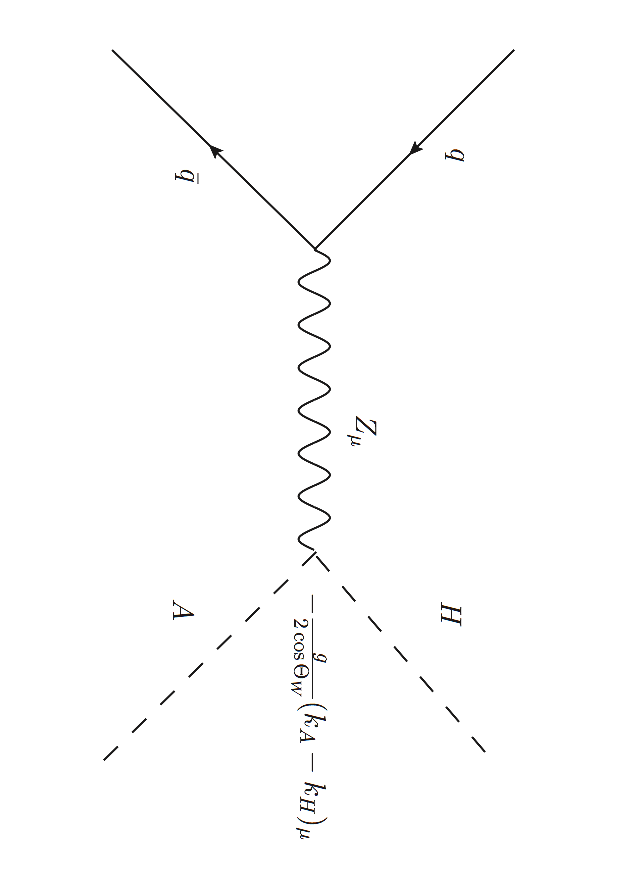
\includegraphics[angle=90,width=0.5\textwidth]{texinputs_app/IDM/ppHA.pdf}
\caption{\label{fig:haprod} Feynman diagram for $Z\,+\,\MET$ final states in the inert doublet model from $H\,A$ production at a hadron collider, with $A\,\rightarrow\,Z\,H$. Production and decay are determined by electroweak SM couplings and masses $m_A,\,m_H$.} 
\end{figure}
